% mnras_template.tex
%
% LaTeX template for creating an MNRAS paper
%
% v3.0 released 14 May 2015
% (version numbers match those of mnras.cls)
%
% Copyright (C) Royal Astronomical Society 2015
% Authors:
% Keith T. Smith (Royal Astronomical Society)

% Change log
%
% v3.0 May 2015
%    Renamed to match the new package name
%    Version number matches mnras.cls
%    A few minor tweaks to wording
% v1.0 September 2013
%    Beta testing only - never publicly released
%    First version: a simple (ish) template for creating an MNRAS paper

%%%%%%%%%%%%%%%%%%%%%%%%%%%%%%%%%%%%%%%%%%%%%%%%%%
% Basic setup. Most papers should leave these options alone.
\documentclass[a4paper,fleqn,usenatbib]{mnras}

% MNRAS is set in Times font. If you don't have this installed (most LaTeX
% installations will be fine) or prefer the old Computer Modern fonts, comment
% out the following line
%\usepackage{newtxtext,newtxmath}
% Depending on your LaTeX fonts installation, you might get better results with one of these:
%\usepackage{mathptmx}
%\usepackage{txfonts}

% Use vector fonts, so it zooms properly in on-screen viewing software
% Don't change these lines unless you know what you are doing
\usepackage[T1]{fontenc}
\usepackage{ae,aecompl}


%%%%% AUTHORS - PLACE YOUR OWN PACKAGES HERE %%%%%

% Only include extra packages if you really need them. Common packages are:
\usepackage{graphicx}	% Including figure files
\usepackage{amsmath}	% Advanced maths commands
\usepackage{amssymb}	% Extra maths symbols

%%%%%%%%%%%%%%%%%%%%%%%%%%%%%%%%%%%%%%%%%%%%%%%%%%

%%%%% AUTHORS - PLACE YOUR OWN COMMANDS HERE %%%%%

% Please keep new commands to a minimum, and use \newcommand not \def to avoid
% overwriting existing commands. Example:
%\newcommand{\pcm}{\,cm$^{-2}$}	% per cm-squared
\newcommand{\blue}{\color{blue}}
\newcommand{\red}{\color{red}}
%%%%%%%%%%%%%%%%%%%%%%%%%%%%%%%%%%%%%%%%%%%%%%%%%%

%%%%%%%%%%%%%%%%%%% TITLE PAGE %%%%%%%%%%%%%%%%%%%

% Title of the paper, and the short title which is used in the headers.
% Keep the title short and informative.
\title[Supernova Gaussianity]{Investigating the Gaussianity of Supernova SALT2 Summary Statistics}

% The list of authors, and the short list which is used in the headers.
% If you need two or more lines of authors, add an extra line using \newauthor
\author[S. R. Hinton et al.]{
Samuel R. Hinton,$^{1}$\thanks{E-mail: \href{samuelreay@gmail.com}}
Alex G. Kim,$^{3}$
Tamara M. Davis,$^{1,2}$
Edward Macaulay$^{1,2}$
\\
% List of institutions
$^{1}$School of Mathematics and Physics, The University of Queensland, Brisbane, QLD 4072, Australia\\
$^{2}$ARC Centre of Excellence for All-sky Astrophysics (CAASTRO)\\
$^{3}$Physics Division, Lawrence Berkeley National Laboratory, 1 Cyclotron Road, Berkeley, CA 94720, USA
}

% These dates will be filled out by the publisher
\date{Accepted XXX. Received YYY; in original form ZZZ}

% Enter the current year, for the copyright statements etc.
\pubyear{2016}

% Don't change these lines
\begin{document}
\label{firstpage}
\pagerange{\pageref{firstpage}--\pageref{lastpage}}
\maketitle

% Abstract of the paper
\begin{abstract}
Write an abstract.
\end{abstract}

% Select between one and six entries from the list of approved keywords.
% Don't make up new ones.
%\begin{keywords}
%keyword1 -- keyword2 -- keyword3
%\end{keywords}

%%%%%%%%%%%%%%%%%%%%%%%%%%%%%%%%%%%%%%%%%%%%%%%%%%

%%%%%%%%%%%%%%%%% BODY OF PAPER %%%%%%%%%%%%%%%%%%

\section{Introduction}

In the years since the discovery of the acceleration of our universe \citep{RiessFilippenko1998, SchmidtSuntzeff1998, PerlmutterAldering1999}, supernova cosmology continued to grow as an important cosmological probe. Recent supernova studies offer far greater statistical power than ever before, systematics are better understood, and the very phenomenon of supernova are described with improved models \citep{GuyAstier2007, ConleyGuy2011, BetouleKessler2014, RubinAldering2015}, and with increased statistical power and model fidelity, systematics are now the limiting constraint in supernova studies \citep{ConleyGuy2011, SuzukiRubin2012, ScolnicRest2014} {\red UPDATE citations, used from Betoule}. In this paper we investigate a potential source of systematics unaddressed in prior studies -- the gaussianity of supernova summary statistics. We perform this investigation within the context of the Dark Energy Survey, which is introduced in Section~\ref{sec:des}. In Section~\ref{sec:motivation} we summarise recent supernova models and analyses, and in Section~\ref{sec:methodology} and Section~\ref{sec:cosmology} we investigate the effect of the assumption of gaussianity on both the supernova distributions obtained and the follow on impact on cosmology.








\section{The Dark Energy Survey}
\label{sec:des}

The Dark Energy Survey \citep[DES,][]{des2005, des2016} is a 5000 sq. deg. photometric redshift survey. The survey will image approximately 300 million galaxies in 5 broadband filters (\textit{grizY}) using the Dark Energy Camera \citep[DECam,][]{FlaugherDiehl2015}. Forty sq. deg. of the sky will be repeatedly images in the \textit{griz} bands for the supernova luminosity distance probe, and is expected to yield observations of approximately 1900 Type Ia supernova up to a redshift of $z=1.2$. {\red No idea where to look for more details on this. On cadence, updated estimates, cadence, difference between shallow and deep fields.}








\section{Motivation}
\label{sec:motivation}

In order to perform a supernova analysis, an underlying Type Ia supernova model must be adopted. The most used model in recent years has been that of the SALT2 model \citep{GuyAstier2007, GuySullivan2010, MosherGuy2014} and in this analysis we restrict our investigations to this model. The SALT2 model characterises the Type Ia spectral energy distribution (SED) as a function of magnitude $x_0$, stretch $x_1$, colour $c$, phase $p$ and wavelength $\lambda$ via
\begin{align}
F(p,\lambda) &= x_0 \left[ M_0(p,\lambda) + x_1 M_1(p,\lambda)\right] \exp\left[c CL(\lambda)\right].
\end{align} 
Thus characterising an individual supernova's magnitude, colour and stretch (and associated covariance) allows recovery of the modelled SED. These summary statistics are used instead of the observed light curves in supernova analyses for computational reasons across many different fitting methodologies. In the Bayesian hierarchical analysis performed on the Unity 2.1 dataset \citep{SuzukiRubin2012} in \citet{RubinAldering2015}, each supernova is described by a latent colour and stretch, which means an analysis with $N$ supernova grows in dimensionality as $2N + x$, where $x$ represents underlying (non-latent) parameters (such as $\Omega_m$). If each supernova has $M$ observations, a full hierarchical model would increase in dimensionality to $(2+M)N + x$, providing vastly increased computational complexity in resolving the underlying posterior surface. In frequentist analyses like that of the Joint Lightcurve Analysis \citep{BetouleKessler2014}, the correlation of all light curve points via the calibration zero points instead leads to computational difficulties in that a covariance matrix of approximate size $MN$ is introduced into the likelihood calculation, which would be prohibitively expensive to invert. Therefore, instead of utilising light curve data directly in cosmological models, light curves are fit to the supernova data to produce summary statistics, and these are then used in cosmology analyses. 

One key assumption when doing this is that these summary statistics are in fact Gaussian in nature. Often this is explicitly assumed in the analysis \citep{MarchTrotta2011, RubinAldering2015}, however it is often implicitly assumed \citep{SullivanGuy2011, SuzukiRubin2012, CampbellDAndrea2013, BetouleKessler2014}. Investigation into asymmetries in the summary statistics are generally limited to asymmetries in the parent colour and stretch distribution \citep{ScolnicRest2014}. {\red More citations.} In our paper we therefore do not investigate biases or asymmetries found in underlying population distributions, but asymmetries and biases in the SALT2 parameter probability surface, and the impact of assuming the Gaussianity of said surface.






\section{Methodology}
\label{sec:methodology}

We begin our investigation by generating supernova light curves for mock supernova in both the DES deep and shallow fields. As prior studies have investigated the effects of parent colour and stretch distributions, we generate all canonical supernova ($x_1 = c = 0$). The supernova are simulated in the \textit{griz} bands with an observational cadence of 5 days, starting from a time $t = -35$, giving 7 observations before the peak to remove the biases introduced by having little data before the luminosity peak {\red CITE}. Weather conditions and moon phase are simulated based on observed DES seeing {\red Cite excel file?}. Simulated light curves undergo a simple selection cut of having at least one observation in any band above a signal to noise of $5$.

We investigate the potential asymmetries in SALT2 summary statistics by fitting the light curves and obtaining summary statistics using different algorithms in the software package \verb|sncosmo| \citep{Barbary2014}. Specifically, we obtain a full posterior surface using our own MCMC fitting methodology, and compare against summary statistics generated using a different MCMC approach (the \verb|mcmc_lc| method in \verb|sncosmo|), nestled sampling (the \verb|nest_lc| method) and minuit (via the \verb|fit_lc| method). The MCMC based algorithm utilises the package \verb|emcee| \citep{ForemanMackey2013}, whilst the nestled sampling is based off \verb|nestle| \citep{Skilling2004, Barbary2015}, and both algorithms should map out the full posterior surface, giving summary statistics from the mean and covariance of that full surface. The third algorithm, invoked via \verb|fit_lc| uses the minuit algorithm \citep{James1975, minuit2015}, and as such is a maximum likelihood estimator and does not map out the full posterior surface. For a Gaussian surface, all three algorithms should agree, however for non-Gaussian surfaces the minuit algorithm will be expected to produce different output. As such, we test the SALT2 probability surfaces for skewness and fit with the four algorithms described previously. The summary statistics are converted into distance modulus via the Philips relation
\begin{align}
\mu = m_B - M + \alpha x_1 - \beta c,
\end{align}
where we adopt the fiducial $\alpha = 0.14$ and $\beta = 3.15$ values from \citet{BetouleKessler2014}. This allows us to directly see the effects of any skewness or non-Gaussianity in any parameter on the cosmologically important distance modulus. We can compare the distributions in $\mu$ for the full posterior surface and for summary statistics, and also verify the skewness of the full distribution of $\mu$. We investigate any shift in $\langle \mu \rangle$, and change in the standard deviation $\sigma_\mu$, binning by redshift, with results illustrated in Figure~\ref{fig:bias_des}. We find strong evidence that, with increasing redshift, the skewness of the SALT2 fit posterior increases, and causes the maximum likelihood estimator to not only produce biased output, but overestimate the uncertainty of the result.
\begin{figure}
	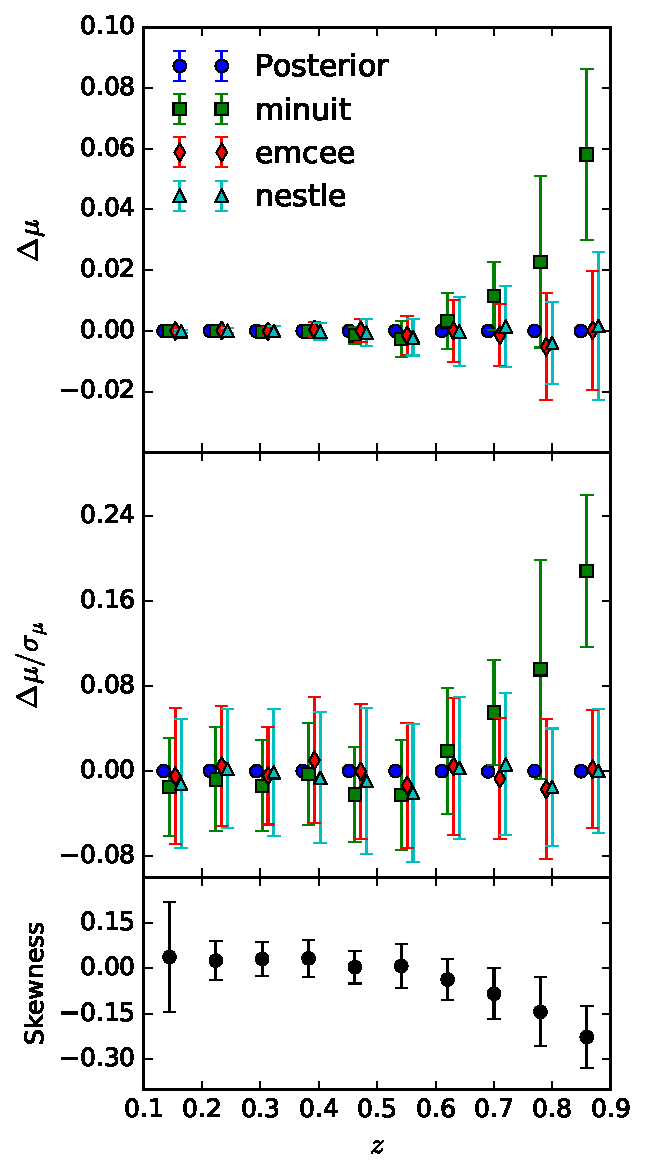
\includegraphics[width=\columnwidth]{../output/bias_dessky.pdf}
    \caption{The bias in distance modulus $\mu$ for observations generated as per the DES shallow field. Supernova results for all algorithms were binned into redshift groups (top two subplots) and the full posterior surface was analysed for skewness (bottom subplot). We find evidence for skewness at higher redshifts, leading to diverging results between mean and maximum likelihood algorithms.}
    \label{fig:bias_des}
\end{figure}
\begin{figure}
	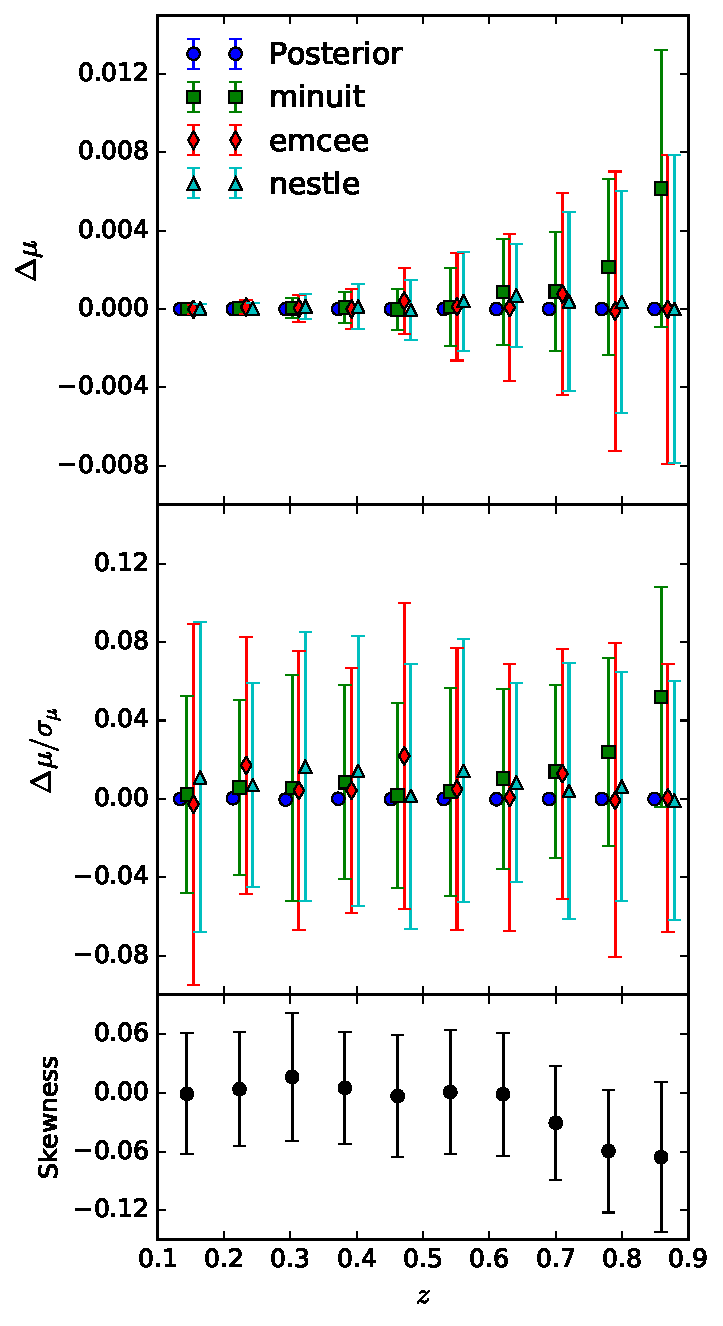
\includegraphics[width=\columnwidth]{../output/bias_dessky_deep.pdf}
	\caption{The bias in distance modulus $\mu$ for observations generated as per the DES deep field. Supernova results for all algorithms were binned into redshift groups (top two subplots) and the full posterior surface was analysed for skewness (bottom subplot). We find evidence for skewness at higher redshifts, however the increased observational time (and subsequent increase in signal-to-noise) results in less biased results than the shallow field.}
	\label{fig:bias_des_deep}
\end{figure}
%The likelihood surface for one of the skewed supernova fits is shown as an example in Figure \ref{fig:example}, where the effect of the skewness is readily apparent.

%\begin{figure*}
%	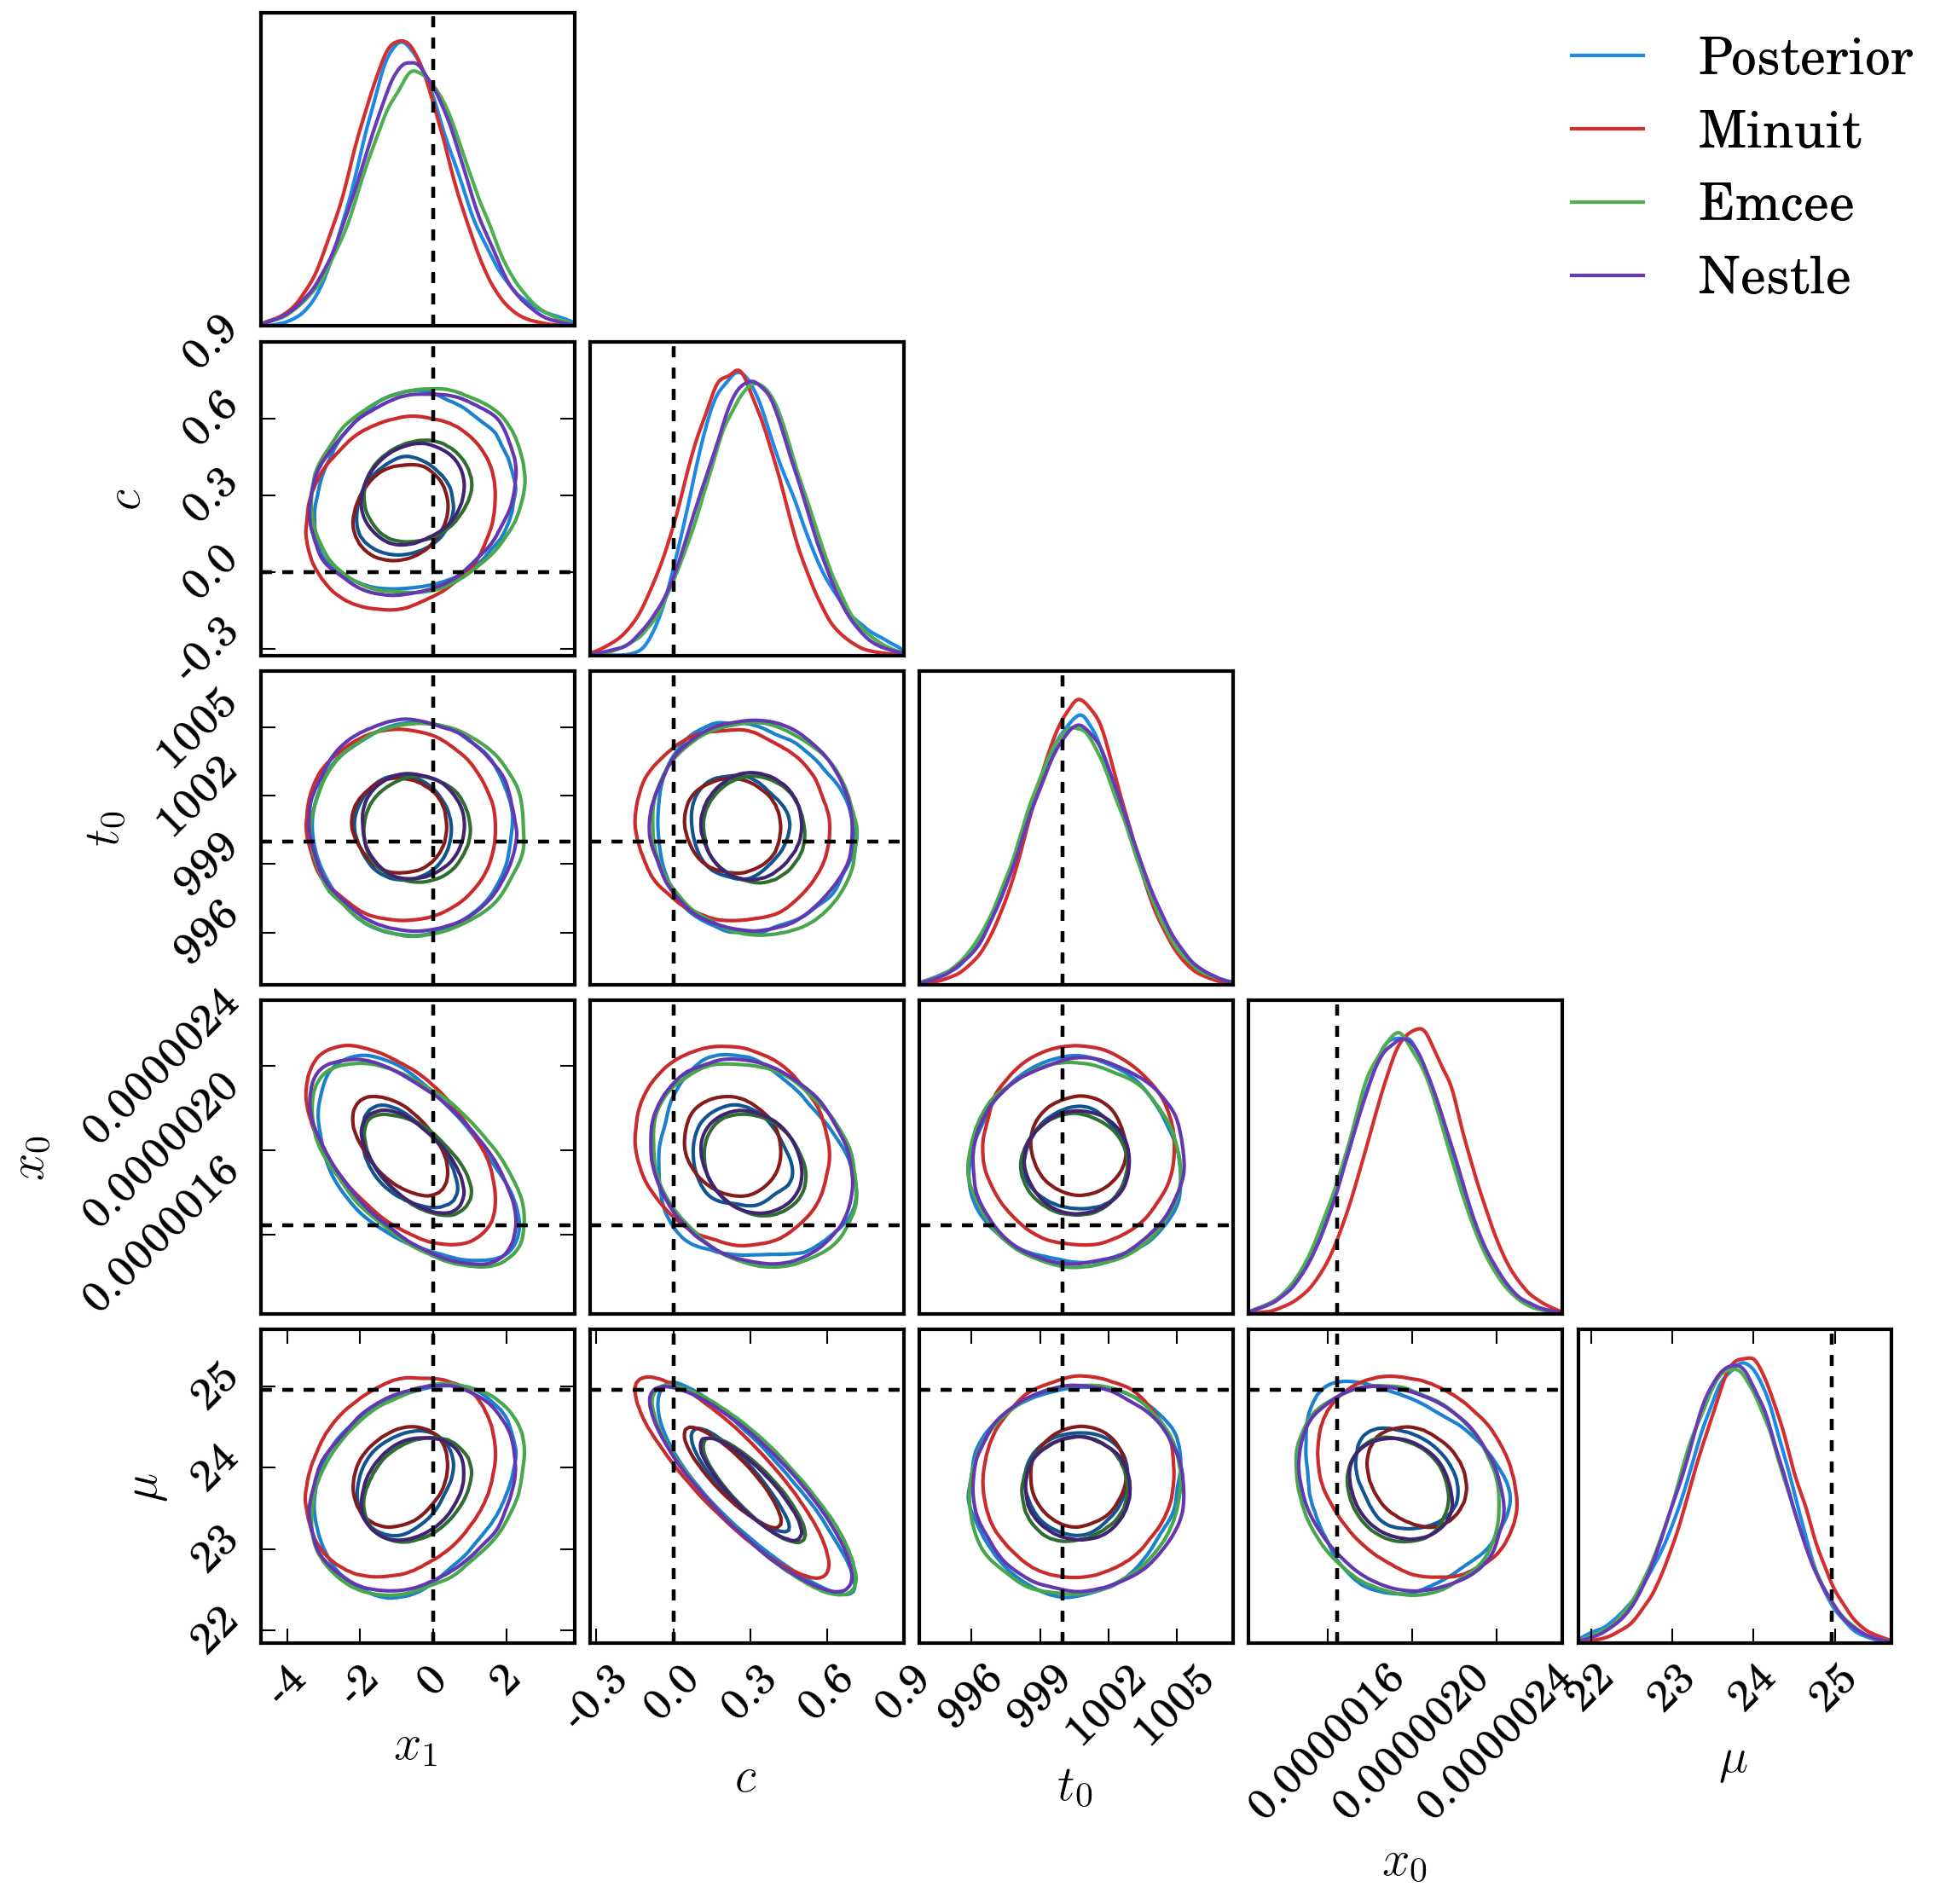
\includegraphics[width=\textwidth]{../output/bias_surface.png}
%	\caption{The posterior surfaces for all algorithms in the SALT2 fit parameters $x_0$, $x_1$, $c$ and $t$, along with the derived value $\mu$. The skewness of the marginalised colour distribution has a significant effect on the skewness of the final $\mu$ distribution, which leads to disagreement between the algorithms used.}
%	\label{fig:example}
%\end{figure*}
To confirm that the skewness is a result of redshift and not simply a result of the general trend of decreasing signal to noise, we plot the skewness as a function of both redshift and signal to noise in Figure \ref{fig:bias_skew}. Interestingly, doing this shows a negative skewness for low redshift, low signal-to-noise light curves, and a positive skewness for high redshift light curves, regardless of signal-to-noise.
\begin{figure}
	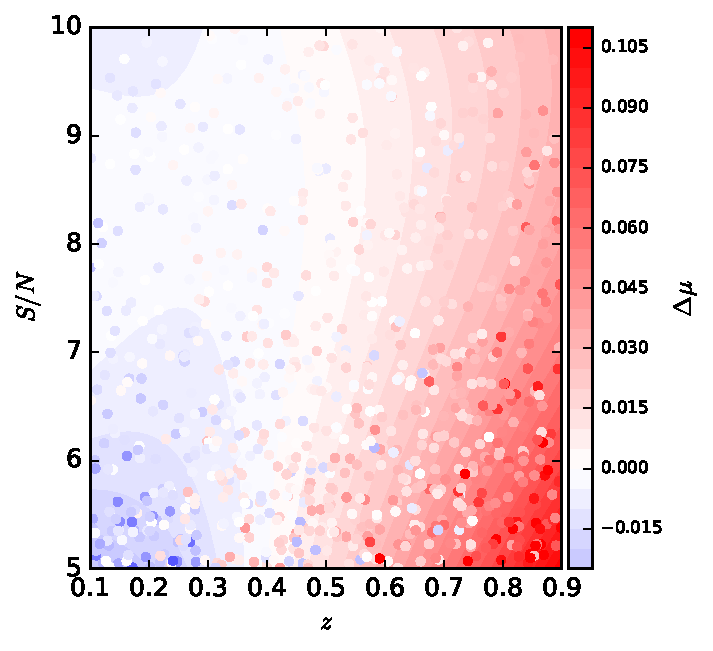
\includegraphics[width=\columnwidth]{../output/bias.pdf}
	\caption{The deviation between the maximum likelihood value for $\mu$ generated by minuit and the mean of the full posterior surfaces. Each point on the plot represents a simulated supernova, with the background surface showing a simple second order polynomial fit to the surface. We can see that, whilst the bias does decrease as signal-to-noise increases, it is still present for the high redsfhit supernova.}
	\label{fig:bias_skew}
\end{figure}
Having confirmed that skewness becomes significant at higher redshift, we now seek to characterise this potential impact on cosmology.


\section{Cosmological Impact}
\label{sec:cosmology}

\subsection{Uncorrected Biases}
For our initial cosmology comparison we generate a thousand supernova for both the shallow and deep fields using simulation cosmology of $\Omega_m = 0.30$, $w = -1.0$, $M_B = -19.3$ and $\sigma_{\rm int} = 0.1$. 10\% of the supernova are drawn from a linear redshift distribution ($0.05 < z < 0.2$) included emulate an external dataset used to constrain the low redshift range of the Hubble diagram, with the remaining 90\% of supernova drawn from a redshift distribution following DES survey volume and $z < 1.2$. The thousand supernova all have the selection effect of having at least one point above a signal-to-noise of 5. We take these thousand supernova and fit their light curves (generated with the same cadence, $t_0$ and weather effects as discussed in the previous section) using both MCMC methods and maximum likelihood methods. As the bias comes from a cut before fitting the light curves, both the set of summary statistics from MCMC and maximum likelihood fitting have the same bias, and any difference between fits to the different sets of summary statistics is thus a product of divergence between the two methodologies and not the cause of selection effects.  We fix $\alpha$ and $\beta$ as done previously, set $\sigma_{\rm int} = 0.1$, and fit a simple model of $\Omega_m$, $w$ and $M_B$.



\begin{figure}
	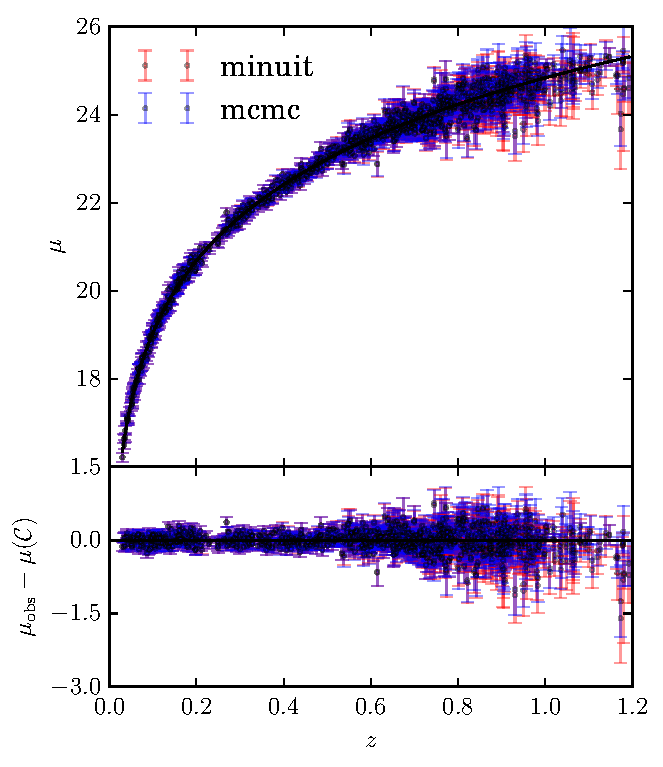
\includegraphics[width=\columnwidth]{../output/obs_cosmology_shallow.pdf}
	\caption{A Hubble diagram sowing the underlying simulation cosmology and the resulting 1000 supernova distance moduli for observations in the DES shallow field. Each supernova is shown twice, once when using summary statistics based in the mean to calculate the distance modulus, and then when using maximum likelihood to generate summary statistics and calculate the distance modulus. Selection effects heavily prune high redshift supernova.}
	\label{fig:obs_cosmology_shallow}
\end{figure}
\begin{figure}
	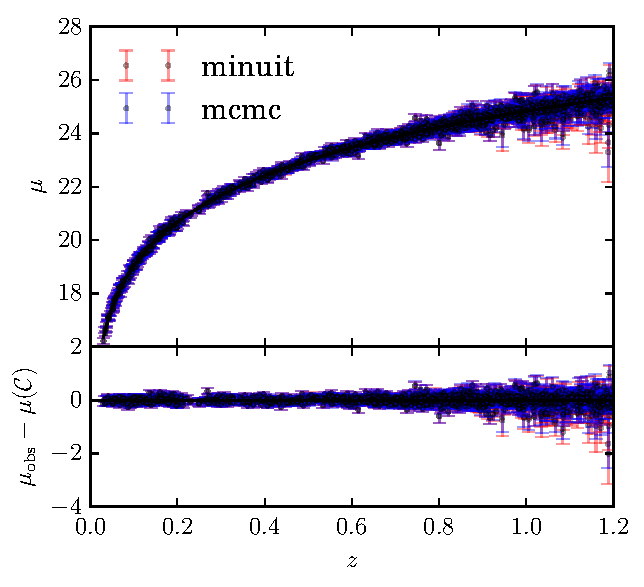
\includegraphics[width=\columnwidth]{../output/obs_cosmology_deep.pdf}
	\caption{A Hubble diagram sowing the underlying simulation cosmology and the resulting 1000 supernova distance moduli for observations in the DES deep field. Each supernova is shown twice, once when using summary statistics based in the mean to calculate the distance modulus, and then when using maximum likelihood to generate summary statistics and calculate the distance modulus. The increased observation in the deep field gives us more high redshift supernova than the shallow field.}
	\label{fig:obs_cosmology_deep}
\end{figure}
\begin{figure}
	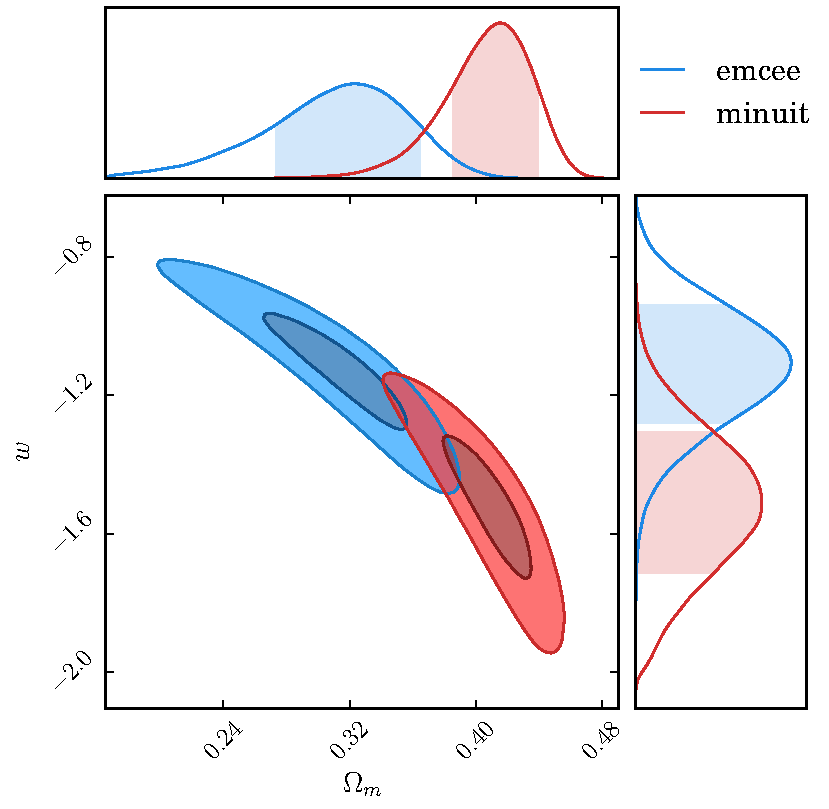
\includegraphics[width=\columnwidth]{../output/comparison_shallow.pdf}
	\caption{{\red Fill out caption in updated figure}}
	\label{fig:comparison_shallow}
\end{figure}
\begin{figure}
	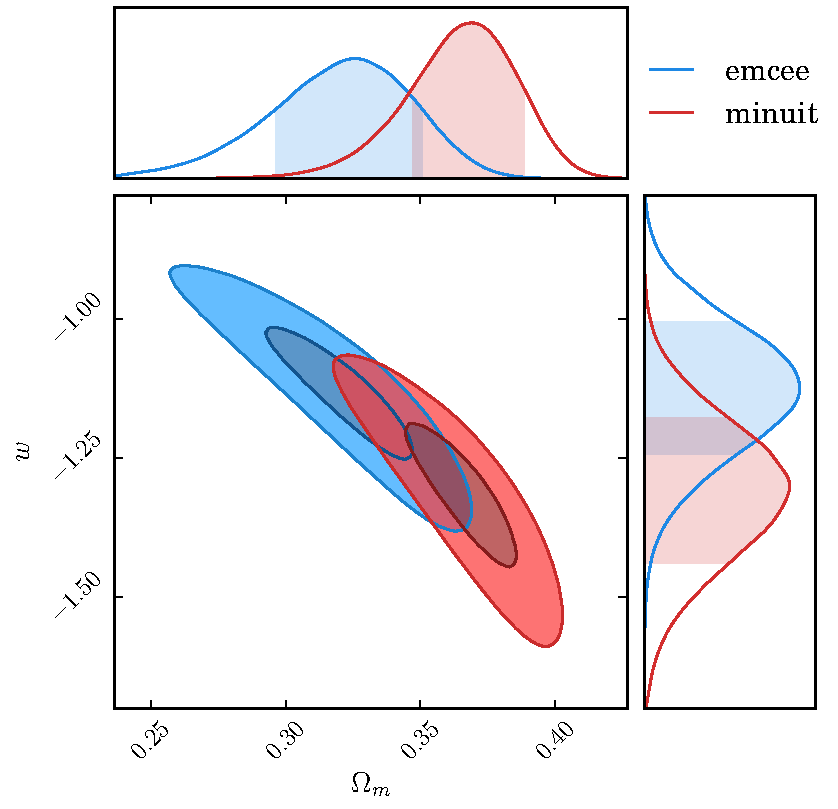
\includegraphics[width=\columnwidth]{../output/comparison_deep.pdf}
	\caption{{\red Fill out caption in updated figure}}
	\label{fig:comparison_deep}
\end{figure}


Figures~\ref{fig:obs_cosmology_shallow} and \ref{fig:obs_cosmology_deep} show the Hubble diagrams (and simulation cosmology) for the shallow and deep simulated supernova respectively. Visible in the diagrams is the systematic bias between the two methodologies at high redshift. Marginalising over the absolute magnitude $M_B$, the cosmological surfaces are presented in Figures~\ref{fig:comparison_shallow} and \ref{fig:comparison_deep}. The shallow field results show a highly significant bias, with even the deep field showing approximately a $1\sigma$ shift when using different methodologies for generating the summary statistics. Table \ref{tab:unbias_comp} shows the marginalised parameter summaries for comparison, and the shift between summary statistics is significant.

\begin{table}
	\centering
	\caption{Comparison between the shallow and deep field cosmology for the mean and maximum likelihood summary statistics.}
	\label{tab:unbias_comp}
    \begin{tabular}{cccc}
       	\hline
       	Model & $\Omega_m$ & $w$ & $M$ \\ 
       	\hline
       	Deep MCMC & $0.317^{+0.027}_{-0.038}$ & $-1.08^{+0.12}_{-0.15}$ & $-19.290^{+0.016}_{-0.017}$ \\ 
       	Deep Max. Like. & $0.362^{+0.024}_{-0.030}$ & $-1.29^{+0.17}_{-0.15}$ & $-19.299^{+0.014}_{-0.020}$ \\ 
       	Shallow MCMC & $0.341^{+0.035}_{-0.051}$ & $-1.17^{+0.19}_{-0.17}$ & $-19.289^{+0.014}_{-0.017}$ \\ 
       	Shallow Max. Like. & $0.426^{+0.018}_{-0.031}$ & $-1.59^{+0.23}_{-0.18}$ & $-19.306^{+0.014}_{-0.018}$ \\ 
       	\hline
    \end{tabular}
\end{table}

The current investigation is not sufficient grounds to claim that any previous cosmology analyses that use maximum likelihood statistics are biased, as this depends strongly on the method of bias correction utilised in prior analyses. For example, methods in which biases are computed from the underlying cosmology may be prone to biases, whilst methods rely on adjusting the data to take into account selection effects calibrated with simulations \citep{KesslerBecker2009, ConleyGuy2011} may be consistent, given simulation SALT2 parameter distributions are drawn from distributions also fit using the observed maximum likelihood summary statistics. Similarly, Bayesian methods, such as modelling selection effects as a Gaussian CDF \citep{RubinAldering2015} are algorithm independent and may correct both sets of summary statistics equally well.

\subsection{Simulation Bias Correction}

Try and do it the Rick Kessler way, verify everything is a-ok

\subsection{Modelled Corrections}

Try and do it the Rubin et al way

\subsection{Cosmological Corrections}

Try and do it the Alex Kim way.


\section{Conclusions}

The last numbered section should briefly summarise what has been done, and describe
the final conclusions which the authors draw from their work.

\section*{Acknowledgements}

The Acknowledgements section is not numbered. Here you can thank helpful
colleagues, acknowledge funding agencies, telescopes and facilities used etc.
Try to keep it short.

%%%%%%%%%%%%%%%%%%%%%%%%%%%%%%%%%%%%%%%%%%%%%%%%%%

%%%%%%%%%%%%%%%%%%%% REFERENCES %%%%%%%%%%%%%%%%%%

% The best way to enter references is to use BibTeX:

\bibliographystyle{mnras}
\bibliography{bibliography}


%%%%%%%%%%%%%%%%%%%%%%%%%%%%%%%%%%%%%%%%%%%%%%%%%%

%%%%%%%%%%%%%%%%% APPENDICES %%%%%%%%%%%%%%%%%%%%%

%\appendix
%\section{Some extra material}
%If you want to present additional material which would interrupt the flow of the main paper, it can be placed in an Appendix which appears after the list of references.

%%%%%%%%%%%%%%%%%%%%%%%%%%%%%%%%%%%%%%%%%%%%%%%%%%


% Don't change these lines
\bsp	% typesetting comment
\label{lastpage}
\end{document}

% End of mnras_template.tex




%SNLS \citep{AstierGuy2006, SullivanGuy2011}
%
%ESSENCE \citep{WoodVaseyMiknaitis2007}
%
%Pan-STARRS \citep{TonryStubbs2012, ScolnicRest2014, RestScolnic2014}
%
%SDSS-II \citep{FriemanBassett2008, KesslerBecker2009, SollermanMortsell2009, LampeitlNichol2010, CampbellDAndrea2013}
%
%Harvard-Smithsonian Center for Astrophysics survey \citep[CfA,][]{HickenChallis2009}
%
%Carnegie Supernova Project \citep[CSP,][]{ContrerasHamuy2010, FolatelliPhillips2010, StritzingerPhillips2011}
%
%Lick Observatory Supernova Search \citep[LOSS,][]{GaneshalingamLi2013}
%	
%Nearby Supernova Factory \cite[SNF,][]{AlderingAdam2002}
%
%HST used in \citep{RiessStrolger2007, SuzukiRubin2012}
%
%Modern results systematic limited \citep{ConleyGuy2011, SuzukiRubin2012, ScolnicRest2014}
%
%Efforts overcome \citep{IvezicSmith2007, RegnaultConley2009, TonryStubbs2012}
